%-----------------------------------------------------------------------------
%
%               Template for sigplanconf LaTeX Class
%
% Name:         sigplanconf-template.tex
%
% Purpose:      A template for sigplanconf.cls, which is a LaTeX 2e class
%               file for SIGPLAN conference proceedings.
%
% Author:       Paul C. Anagnostopoulos
%               Windfall Software
%               978 371-2316
%               paul@windfall.com
%
% Created:      15 February 2005
%
%-----------------------------------------------------------------------------


\documentclass[]{sigplanconf}

% The following \documentclass options may be useful:
%
% 10pt          To set in 10-point type instead of 9-point.
% 11pt          To set in 11-point type instead of 9-point.
% authoryear    To obtain author/year citation style instead of numeric.

\usepackage{graphicx}
\usepackage{amsmath}
\usepackage{hyperref}
\usepackage{graphicx}

\newcommand{\squishlist}{\begin{list}{$\bullet$}
  {\setlength{\itemsep}{0pt}
    \setlength{\parsep}{3pt}
    \setlength{\topsep}{3pt}
    \setlength{\partopsep}{0pt}
    \setlength{\leftmargin}{1.5em}
    \setlength{\labelwidth}{1em}
    \setlength{\labelsep}{0.5em}}}

\newcommand{\squishend}{\end{list}}

\begin{document}

\conferenceinfo{Sprezzatech}{Aug 6, Atlanta.} 
\copyrightyear{2013} 
\toappear{Copyright is held by the author.\\
\textit{Sprezzatech} Aug 6, Atlanta.}
%\authorpermission
%\titlebanner{CS8803DC, Spring 2010, Georgia Institute of Technology}        % These are ignored unless
%\preprintfooter{Dynamic Translation for Intel's Loop Stream Decoder}   % 'preprint' option specified.

\title{Streaming Audio in the Gulf of Guinea}
\subtitle{Categorizing and Delivering Nigeria's Music}

\authorinfo{Nick Black}
           {nick.black@sprezzatech.com}

\maketitle

\begin{abstract}
Nigeria presents unique challenges and opportunities to mobile internet streaming
services. Major services such as Pandora\cite{pandoracountries} and
Spotify\cite{spotifycountries} have no presence in West Africa. Its multiethnic
and vivid culture produced worldwide sensations: Chinua Achebe, Wole Soyinka,
Chris Ofili, and ``Nollywood'', the hub of African cinema. Nigeria
was recognized as a ``Next Eleven'' country by Goldman-Sachs\cite{n11},
and is predicted by \textit{The Economist} to be the world's third most-populous
nation by 2050\cite{economist}. Cellular penetration approaches 70\% of the population\cite{nigeriamobile},
provides 70\% of the nation's internet access, and is expected to increase
dramatically following the dissolution and sale of the moribund, state-run
NITEL (Nigeria Telecommunications, Limited)\cite{reutersnitel}. This cellular access,
however, suffers reliability, quality-of-service, and capability issues, with
many users adopting multiple carriers\cite{reuterssims}. Furthermore, nascent
Nigerian streamers such as iROKING and Gbedu.FM have not introduced 
automated psychoacoustic categorization of African music. We investigate the
feasibility of cost-effective streaming and categorization of Nigerian music.
\end{abstract}

\category{ITU}{Region 1}{Nigeria}

\terms
Nigerian cellular, streaming music

\keywords
Nigeria, streaming, psychoacoustics

\section{Introduction}
Streaming music requires three technological capabilities:
\begin{itemize}
\item Bandwidth sufficient to deliver high-quality audio. The server side
	requires bandwidth for a great many concurrent streams: bandwidth
	requirements will generally follow the product of the number of streams
	and the streams' bit rates.
\item A delivery system capable of maintaining low jitter across the length
	of a song, and which does not introduce high latencies between songs.
\item The ability to categorize large amounts of music for the purposes of
	music discovery and automatic playlist generation. Music discovery
	is assisted by categorization refinement, while automatic playlist
	generation relies on very simple evaluations.
\end{itemize}
The first two capabilities are systematic, real-time quality-of-service
demands. The third can be performed offline, wholly on the server side.

\section{Telecommunications in Nigeria}
Nigerian Internet access is representative of West Africa and radically
distinct from that of North America and Europe.
\begin{itemize}
\item	\textbf{The majority of Nigeria's transnational traffic involves
	oceanic carriers.}
	Africa lacks a pan-continental ``backbone'' as measured by in-continent
	IXP (Internet eXchange Point) traffic\cite{pingdom}. IXPs are fragmented
	into three major hubs (South Africa, the East African islands, and
	Northern Africa); outside these hubs, few backbones cross national
	borders (the World Bank has extended a loan for the
	Central Africa Backbone Project, connecting ECCAS
	states\footnote{The Adaptable Program Loan (APL) for Phase 1 will
	connect Economic Community of Central African States Chad, Cameroon,
	and the Central African Republic\cite{apl1a}.}). Bandwidth
	into and out of Nigeria is thus paced by underwater cable laying, and
	subject to long-path latency. Nigeria has no true Tier 1 provider\footnote{The only
	Tier 1 ISPs in Africa operate from South Africa and Ghana\cite{drpeering}, though
	Suburban Telecom\cite{suburban}, Main One and Globanet all boast
	Tier 1 partners.}.
	
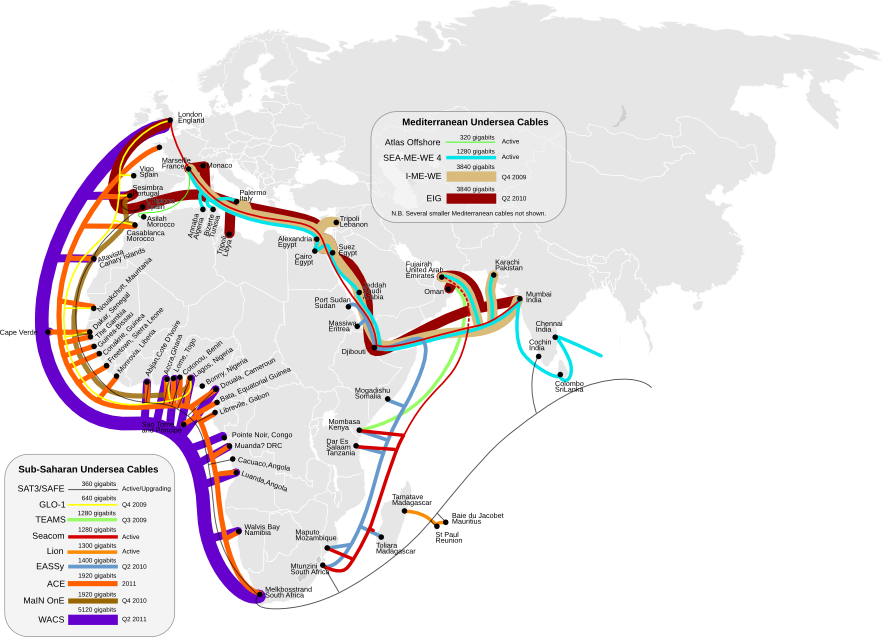
\includegraphics[scale=.4]{subsahara.png}

\item \textbf{The majority of Nigeria's intranational traffic involves
	cellular carriers.} Through 2009, international fiber bandwidth consisted solely of state monopoly
	NITEL's SAT-3/WASC access\cite{backbone}; reliability problems and cost drove 30\%
	of Internet users to high-latency, low-throughput
	Very Small Aperture Terminal (VSAT) parabolic satellite service.
	Numerous West African cables have since been added, including
	Globacom's Glo-1, MTN's Main One, Orange's ACE, and Alcatel-Lucent's WACS
	(Nigeria is not connected to ATLANTIS-2), with landing points at
	Lagos and Bonny Island. IXPN (formerly NIXP) offers 10Gbps IXPs at
	Lagos's NET House Colo and Vicroria Island's Medallian Colo\cite{ixpn}.
	Fibre backbones into the heart of Nigeria are underdeveloped; the NCC's
	Wire Nigeria Project and State Accelerated Broadband Initiative\cite{nccwire}
	aimed to subsidize development, but the majority of Nigeria's fixed
	lines have been implemented using wireless technology\cite{fixedline}.

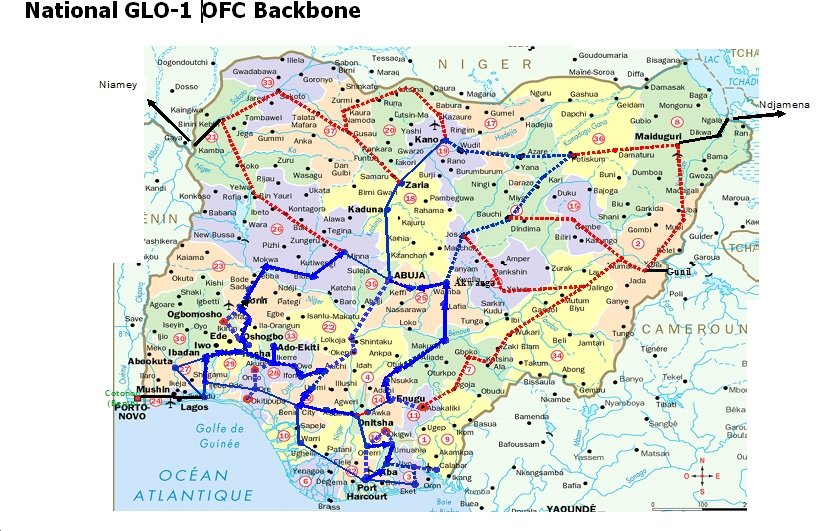
\includegraphics[width=\linewidth]{glo-1.jpg}
\end{itemize}

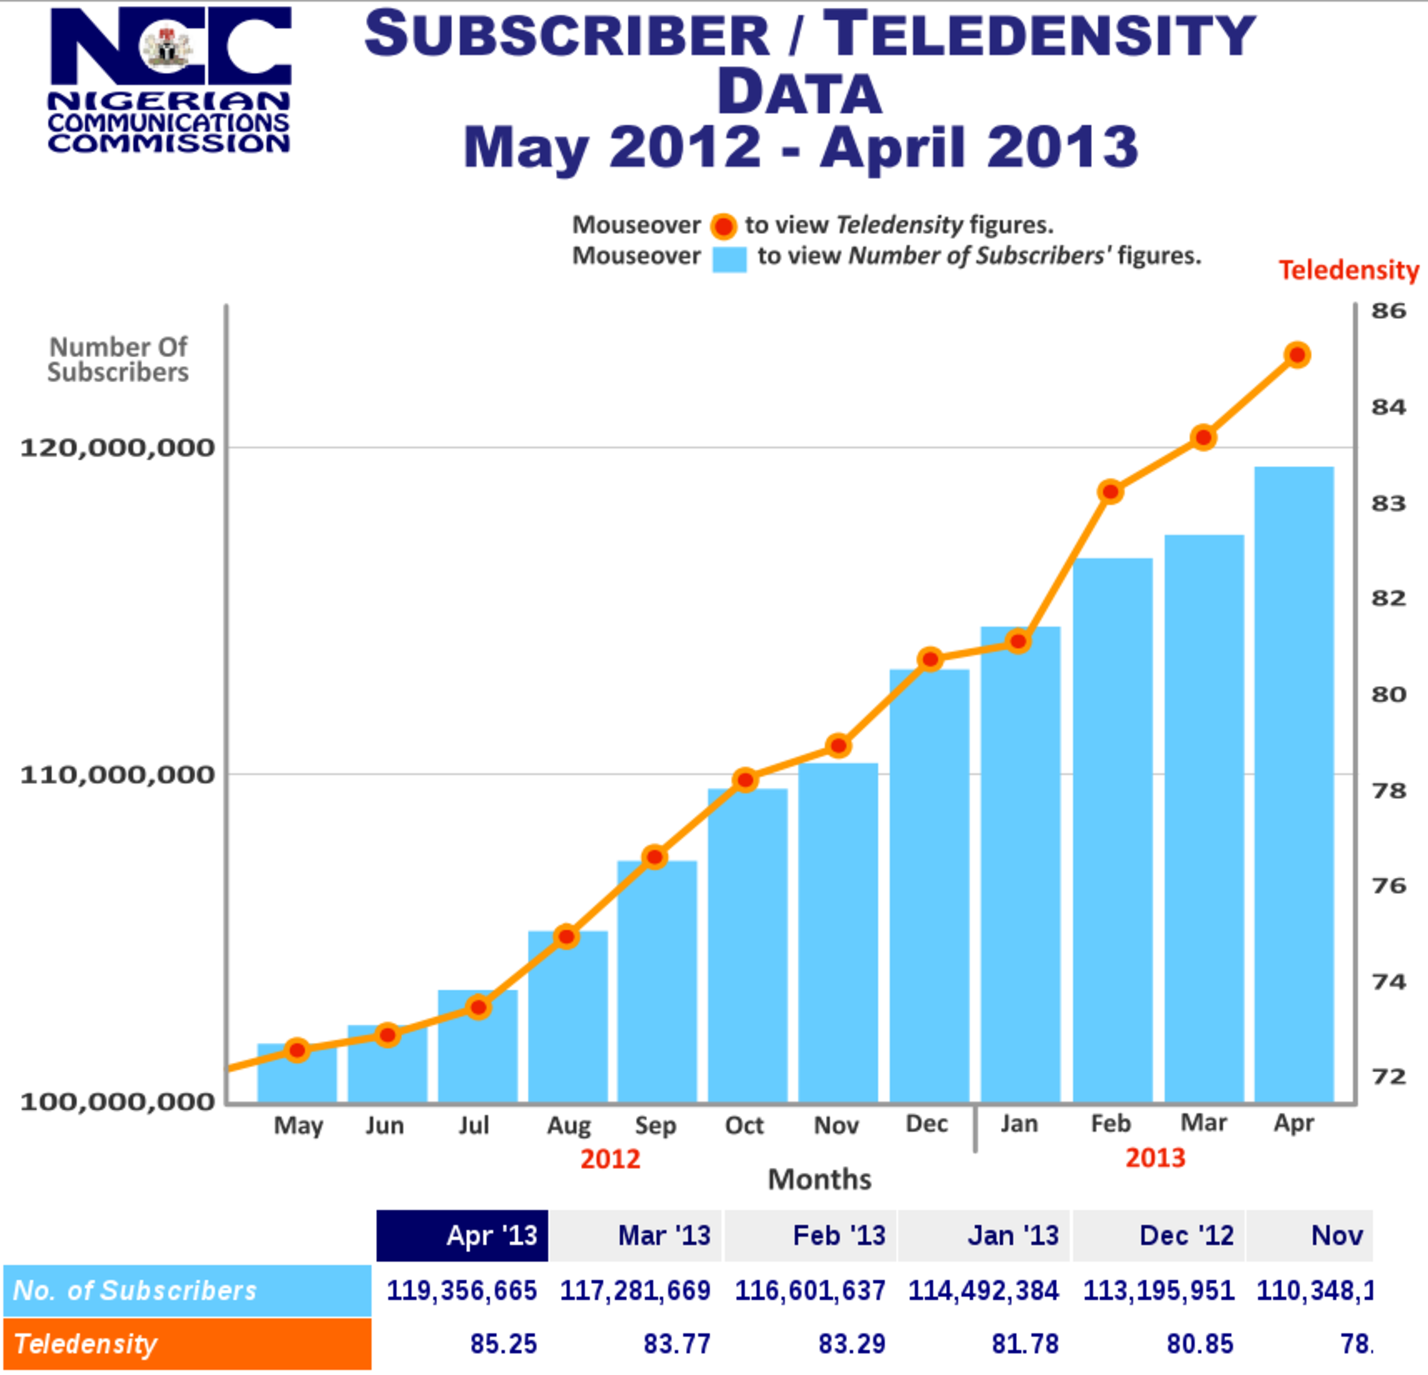
\includegraphics[width=\linewidth]{ncc.pdf}
\\


This is wrongheaded.

While it is true that streaming instructions (in the case of Conroe) or $\mu$ops
(in the case of Nehalem) from the Loop Stream Detector bypasses several pipeline stages,
this does not, by itself, represent a gain in throughput. At a saturated steady
state, IPC is independent of pipeline length. The LSD applies only to tight
loops---precisely the sections most easily benefited by branch prediction,
large data caches, advanced prefetching and extensive speculation. In short,
it targets code for which Intel has already spent a decade adding hardware
support (as noted earlier, the LSD \textit{can} remedy certain decoding
perversions specific to the x86 architecture).

The LSD would be highly relevant to research on optimizing for power, were it
not for the facts that:
\squishlist
\item It is present only on energy-hungry high-end x86 processors, poor fits for
systems designed to conserve power.
\item It is only so effective at reducing power consumption due to the large
transistor budget required for high-speed x86 instruction decoding; a classic
RISC processor could not reap nearly such significant benefits.
\squishend
Whether or not the Loop Stream Detector will emerge as the focus of academic
research is debatable. This paper appears to be the first investigation
of dynamic translation for the explicit purpose of engaging the LSD.
\appendix

\bibliographystyle{abbrvnat}
% The bibliography should be embedded for final submission.
\bibliography{nigeria}
\end{document}
